% 匿名化示例：名称、权利人和日期均为演示值，不代表真实申请事实。
\documentclass[UTF8,fontset=windows,zihao=-4]{ctexart}

\usepackage[a4paper,left=22mm,right=22mm,top=24mm,bottom=22mm,headheight=18pt]{geometry}
\usepackage{graphicx}
\usepackage{array}
\usepackage{booktabs}
\usepackage{longtable}
\usepackage{tabularx}
\usepackage{enumitem}
\usepackage{fancyhdr}
\usepackage{hyperref}
\usepackage{caption}
\usepackage{float}
\usepackage{setspace}
\usepackage{xcolor}

\graphicspath{{figures/}}
\hypersetup{hidelinks}
\captionsetup{font=small,labelfont=bf}
\setstretch{1.35}
\setlength{\parindent}{2em}
\setlength{\parskip}{0.2em}
\setlist{nosep,leftmargin=2.2em}
\renewcommand{\arraystretch}{1.25}

\newcommand{\softwareName}{天平实验训练示例}
\newcommand{\softwareVersion}{V1.0}
\newcommand{\copyrightOwner}{示例著作权人}

\newcommand{\menu}[1]{\textbf{#1}}
\newcommand{\api}[1]{\nolinkurl{#1}}
\newcommand{\redblank}[1]{{\color{red}\underline{\hspace{#1}}}}

\pagestyle{fancy}
\fancyhf{}
\fancyhead[L]{天平实验训练示例 V1.0}
\fancyhead[R]{第 \thepage 页}
\fancyfoot[L]{著作权人：\copyrightOwner}
\fancyfoot[R]{使用说明书}
\renewcommand{\headrulewidth}{0.4pt}
\renewcommand{\footrulewidth}{0.4pt}

\begin{document}

\begin{titlepage}
  \centering
  \vspace*{28mm}
  {\zihao{1}\bfseries \softwareName\par}
  \vspace{8mm}
  {\zihao{2}\bfseries \softwareVersion\ 使用说明书\par}
  \vspace{18mm}
  {\zihao{4} 计算机软件著作权登记文档鉴别材料\par}
  \vfill
  \begin{tabular}{>{\bfseries}p{36mm}p{86mm}}
    软件全称 & 天平实验训练示例 \\
    软件版本 & V1.0 \\
    开发完成日期 & 2026 年 1 月 1 日 \\
    文档类型 & 使用说明书 \\
    适用对象 & 实验练习者、教师及软件使用人员 \\
  \end{tabular}
  \vfill
  {\zihao{-4} 本说明书适用于 \softwareName\ \softwareVersion，说明软件功能组成、运行环境、实验操作、评分规则、主要界面和数据保存方法。\par}
\end{titlepage}

% 目录局部使用较紧凑字号和单倍行距，正文版式保持原模板。
\begingroup
\small
\setstretch{1}
\setlength{\parskip}{0pt}
\tableofcontents
\endgroup
\clearpage

\section{软件概述与功能组成}

系统围绕托盘天平实验的准备、称量、读数及收尾过程构建交互练习。用户通过器材按钮、工具选择和滑杆改变虚拟实验状态；天平指针、托盘倾斜、阶段得分及操作提示随服务器返回结果更新。

\begin{longtable}{@{}p{38mm}p{114mm}@{}}

\toprule

功能 & 操作与结果 \\

\midrule

\endfirsthead

\toprule

功能 & 操作与结果 \\

\midrule

\endhead

实验操作台 & 检查器材、归零、调平、放置物体、增减砝码、调整游码和记录读数。 \\

过程评价 & 逐项记录八环节完成情况，输出即时纠错信息及累计分数。 \\

实验报告 & 结束当前轮次后查看得分、读数、事件及违规记录，并打印报告。 \\

历史记录 & 查看已有轮次，读取其报告和导出记录。 \\

操作指南 & 查看实验流程和评分说明，按提示完成规范操作。 \\

\bottomrule

\end{longtable}

\subsection{使用边界}

本版本为纯本地交互练习软件，不接入摄像头、物联网天平、视觉识别模型或在线大模型。软件记录来自用户在界面上的操作，不从视频推断实验动作。

\subsection{使用组织}

系统无需注册账号，由当前电脑上的使用者进行操作。实验数据保存在本地文件中；同一数据目录内的轮次共同出现在历史记录中。演示轮次使用演示来源标记，与普通练习来源区分。

\subsection{一次操作的数据流}

界面与本机服务通过 HTTP 和 JSON 交换数据，操作按下列顺序处理：

\begin{enumerate}

\item 浏览器读取当前轮次，展示器材状态与已有分数。

\item 用户点击器材按钮或调节滑杆，界面提交动作类型与参数。

\item 服务检查轮次是否仍在进行中，并验证参数类型及取值范围。

\item 规则模块检查前置步骤、器材位置和工具，更新状态及操作事件。

\item 分项完成标记按满足条件的项目更新，同一项目只计分一次。

\item 服务串行写入临时 JSON 文件，再替换已保存的数据文件。

\item 保存成功后返回新状态，界面同步更新天平、评分与提示。

\item 结束实验后，报告与导出文件使用同一份归档记录。

\end{enumerate}

\subsection{记录的组成}

每轮实验形成独立记录，导出时保留以下信息：

\begin{itemize}

\item 轮次编号：系统生成唯一编号，用于区分名称相同的实验。查询报告或导出JSON后，先核对编号，再比较其他字段，避免把不同轮次的结果混用。

\item 记录来源：区分自主练习和演示记录。新建实验时选择来源，历史列表保留该标记；演示轮次用于展示功能，不能解释为真实学生成绩。

\item 起止时间：创建时保存开始时间，结束时保存归档时间。进行中的实验与已经结束的记录具有不同状态，结束后可继续查看报告，但不再接收实验动作。

\item 器材状态：保存托盘位置、砝码、游码、螺母和所选工具。刷新页面后由服务端返回保存的状态，器材整理后的当前状态与读数时的测量快照分别记录。

\item 测量快照：正确读数时保存砝码合计、游码示值和读数。报告据此说明测量组成，即使之后执行整理归位，也能够核对原来的质量读数。

\item 操作事件：逐次保存时间、动作反馈和是否属于违规提示。纠正操作后先前的提示仍会保留，可结合分项结果回顾本轮实验是直接完成还是纠正后完成。

\end{itemize}

\section{运行环境与本地启动}

\begin{longtable}{@{}p{38mm}p{114mm}@{}}

\toprule

项目 & 配置 \\

\midrule

\endfirsthead

\toprule

项目 & 配置 \\

\midrule

\endhead

操作系统 & Windows 本地运行环境 \\

服务运行时 & Node.js 22.18 或更高版本 \\

访问工具 & 支持现代 JavaScript 的 Edge 或 Chrome 浏览器 \\

访问地址 & http://127.0.0.1:3187 \\

网络范围 & 服务绑定 127.0.0.1，仅本机访问 \\

数据介质 & 可写的本地项目目录 \\

\bottomrule

\end{longtable}

\subsection{首次准备}

将交付压缩包完整解压到可写目录，保留目录层级。确认已安装可用的 Node.js。交付包包含前端构建产物，日常启动无需安装开发依赖。需要修改源码后重新构建时，运行“安装依赖.cmd”，等待安装和构建成功；依赖安装可能需要联网。

\subsection{启动系统}

双击“启动.cmd”。脚本启动本地服务后，在浏览器访问 http://127.0.0.1:3187。保留项目中的服务文件、构建产物和数据目录，避免在运行过程中移动或改名。

\subsection{停止系统}

操作结束后先结束需要保存报告的轮次，再执行“停止.cmd”。关闭浏览器页面不等同于停止本地服务。再次启动后，可以通过历史记录读取此前保存的实验。

\subsection{端口占用}

如果提示端口已被使用，先检查本系统是否已经启动，并尝试访问上述地址。若是其他程序占用端口，停止已确认的冲突程序后再启动，不要任意终止未知进程。

\subsection{启动后的检查顺序}

按以下项目确认程序和数据都已就绪：

\begin{enumerate}

\item 核对地址栏为本机 127.0.0.1，默认端口为 3187。

\item 页面顶部应显示完整软件名称及 V1.0 版本。

\item 顶部连接状态应为“本地服务已连接”。

\item 导航应能切换实验台、实验记录和实验指南。

\item 新建轮次时填写名称，并选择自主练习或演示来源。

\item 开始后检查八个项目均未完成，初始分数为零。

\item 执行器材检查，应看到对应反馈和第一项得分。

\item 刷新页面，确认刚才的器材检查和分数仍然存在。

\item 若连接失败，查看 .runtime/server-error.log 中的启动信息。

\item 如果记录文件损坏，先保留原文件，再用已知备份恢复。

\end{enumerate}

\subsection{从源码重新构建}

需要修改软件时，使用完整源码包中的源文件，并在解压后的项目目录执行构建命令。源程序PDF用于查看鉴别材料，开发时直接编辑工程中的TypeScript、HTML和CSS文件。

\begin{enumerate}
\item 安装Node.js 22.18或更高版本，并确认终端可以执行node和npm。
\item 打开源码目录，核对package.json与package-lock.json均存在。
\item 执行\api{npm ci}，按锁定文件安装依赖；安装时可能需要联网。
\item 在src目录修改界面及样式，在server目录修改本机服务及实验规则。
\item 修改后执行\api{npm test}，检查现有规则、接口和数据保存测试结果。
\item 执行\api{npm run build}，完成类型检查并生成dist生产页面。
\item 构建成功后执行\api{npm start}，在浏览器打开本机3187端口。
\item 检查新建轮次、器材操作、评分、报告和历史记录是否符合预期。
\end{enumerate}

代码修改后应同步检查说明书与截图。备份数据后再进行会影响记录结构的调整，保留源文件、依赖锁定文件和对应版本的构建产物，以便重建及核对。

\section{界面与实验准备}

\begin{figure}[!htbp]\centering
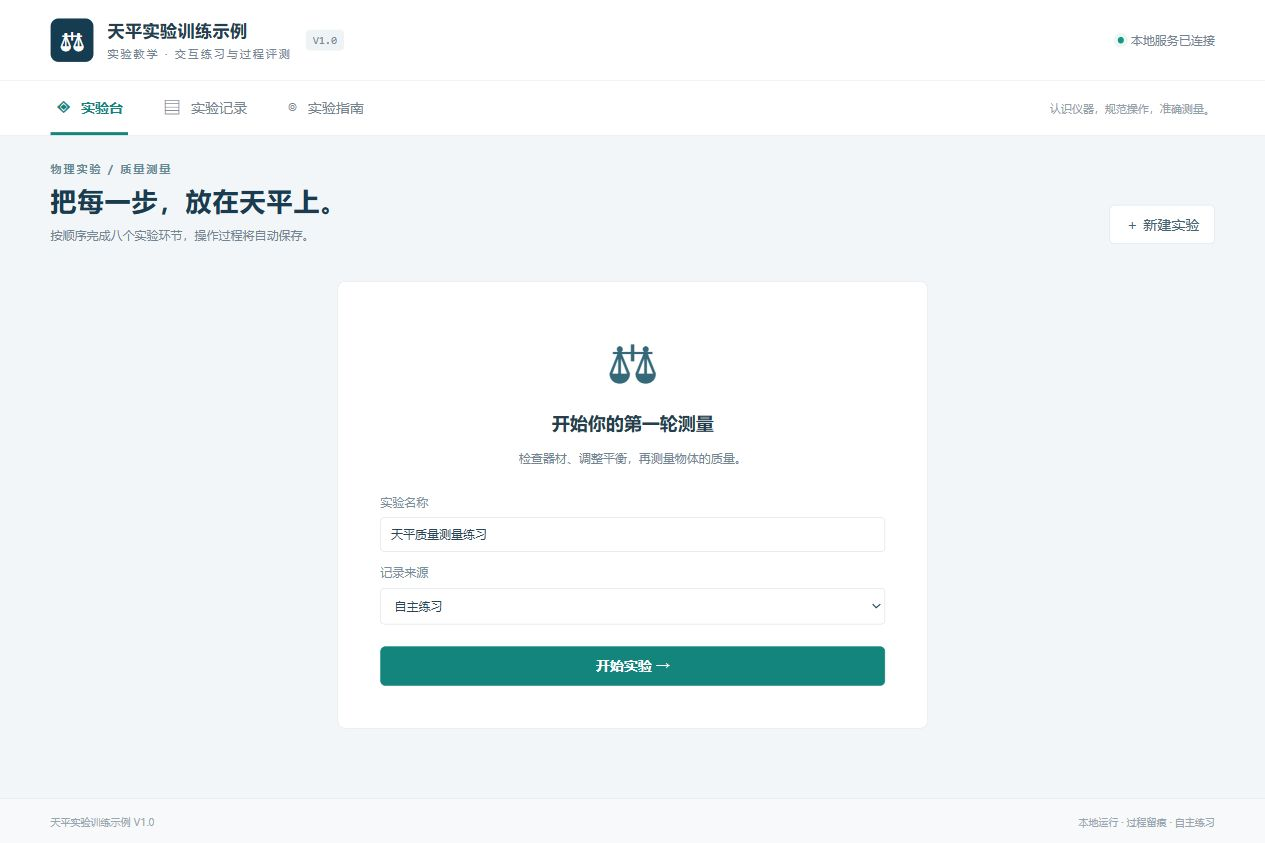
\includegraphics[width=0.95\linewidth,height=90mm,keepaspectratio]{01-home.png}
\caption{实验操作台初始界面}
\end{figure}

操作台集中显示天平、器材控制、评分进度和最新反馈。开始操作前，应查看当前轮次名称及状态，确认所操作的是本次练习。主导航用于在实验操作、历史记录与操作指南间切换。

\subsection{检查器材}

首先使用器材检查控件完成检查。系统记录检查事件并更新第一项得分。重复执行已完成的检查不会重复增加分数。随后将游码移至零刻度，确认左右托盘均无物体和砝码，再调整天平。

\subsection{输入方法}

按钮可用鼠标点击，也可通过 Tab 聚焦后用 Enter 或空格激活。滑杆获得焦点后可用方向键微调。读数框按克输入数值，保留一位小数。每次操作后先查看反馈，再继续下一步。

\section{归零调平与规范操作}

\begin{figure}[!htbp]\centering
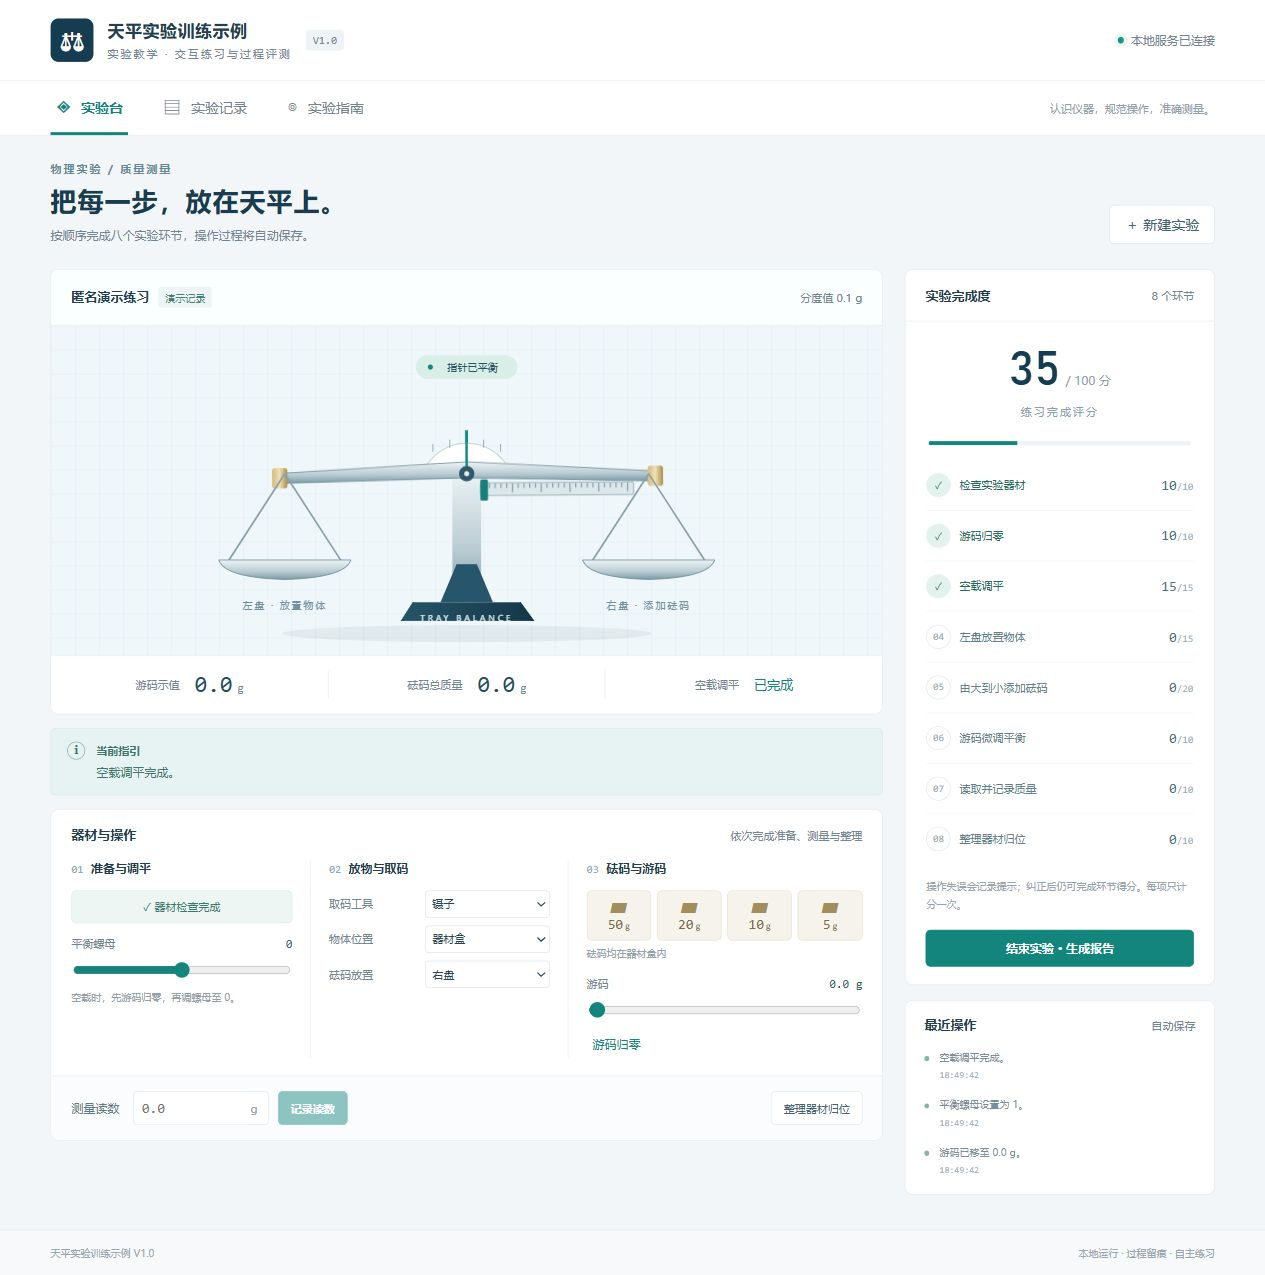
\includegraphics[width=0.95\linewidth,height=125mm,keepaspectratio]{02-prepared.png}
\caption{归零及空载调平后的实验状态}
\end{figure}

游码归零后，在左右盘均为空的条件下调整平衡螺母。指针回到中心且系统确认空载调平后，才能开始称量。空载调平与称量时通过砝码、游码达到平衡属于不同操作。

\subsection{放置物体及选择工具}

将待测物体放在左盘。选择镊子后向右盘添加砝码，并遵循由大到小的顺序。若放错位置，先将相应器材取回，再按正确位置放置。

\subsection{纠错原则}

在前置步骤未完成、物体放错托盘或使用不合适工具时，系统返回具体提示并记录违规事件。根据提示修正操作后可以继续练习；违规不会以负分扣除已获得的分数。

\section{称量与读数}

\begin{figure}[!htbp]\centering
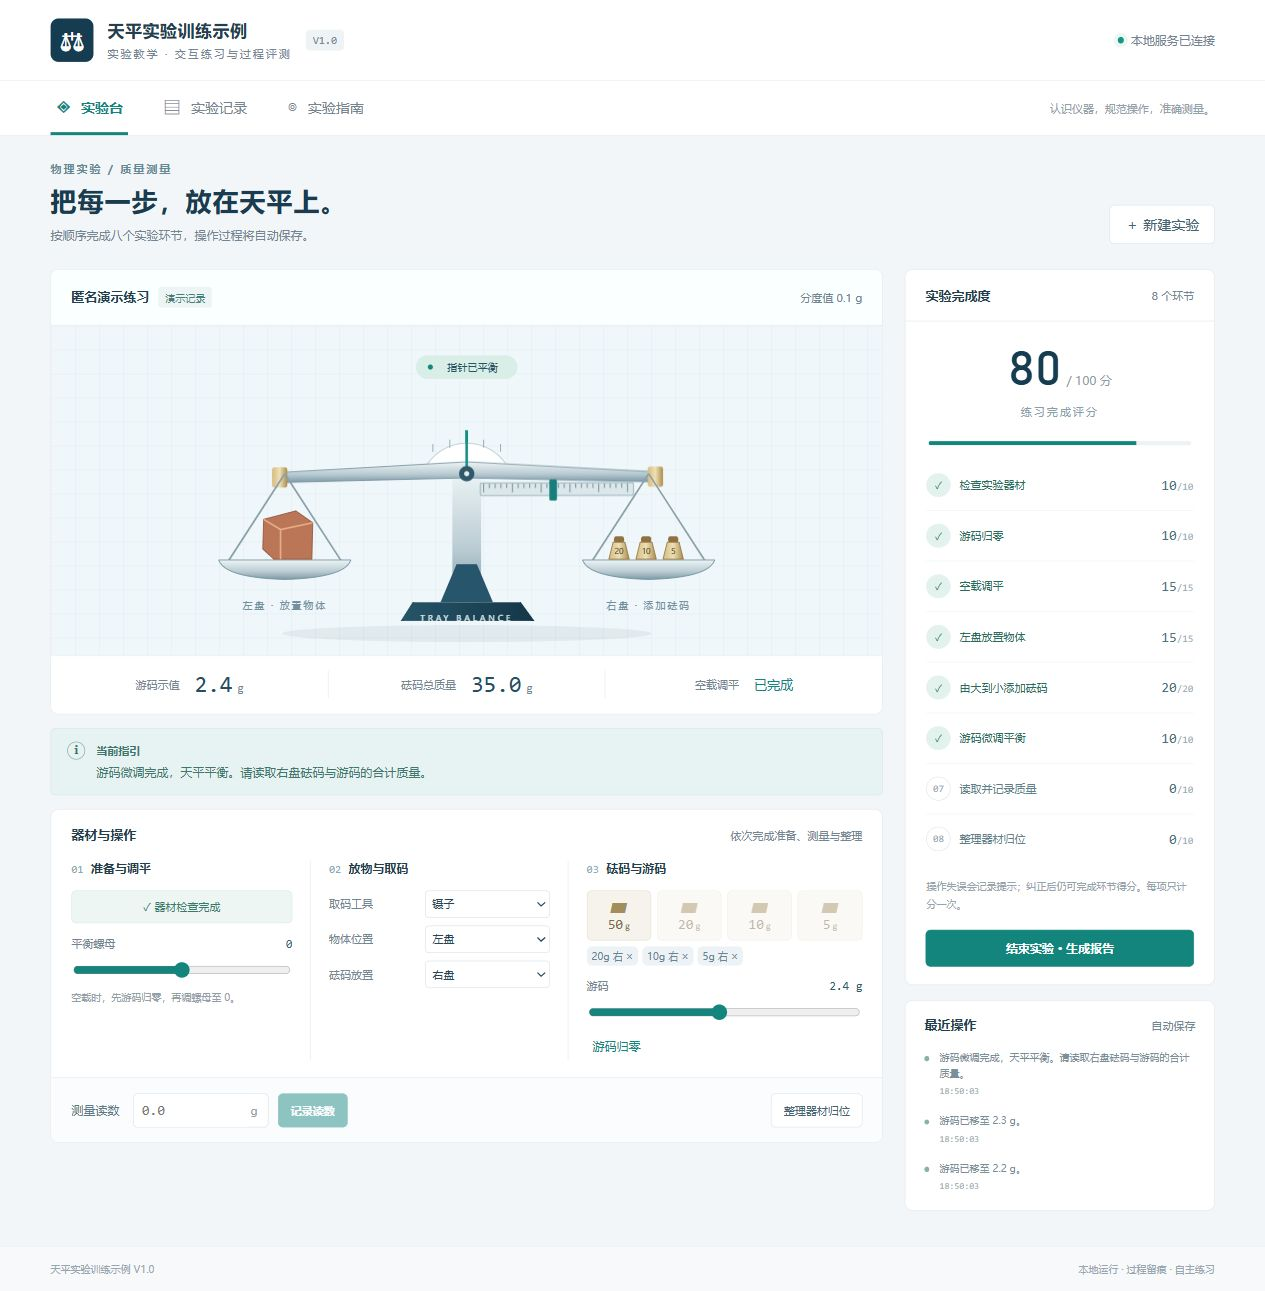
\includegraphics[width=0.95\linewidth,height=125mm,keepaspectratio]{04-balanced.png}
\caption{正确放置物体并调整砝码及游码后的平衡状态}
\end{figure}

使用右盘砝码接近物体质量，再调整游码消除剩余差值。根据当前指针和状态提示判断是否已经平衡，不要仅凭某个按钮已被点击判断实验完成。

\subsection{数值单位}

界面以克为单位显示一位小数，读数框最多输入一位小数。系统采用整数十分之一克计算，避免小数误差影响平衡判断。

本版本固定物体质量为 37.4 g，提供 50、20、10、5 g 砝码各一枚；游码范围 0.0 至 5.0 g，步进 0.1 g。示例使用 20、10、5 g 砝码加 2.4 g 游码。螺母范围 -5 至 5，空载调平时归零。

\subsection{提交读数}

在正确调平、左物右码且达到平衡的条件下，将右盘砝码总质量与游码示值相加，把结果填入读数框并提交。未平衡或读数错误时先修正，不会将错误输入作为正确完成结果。

\section{八环节评分规则}

\begin{longtable}{@{}p{43mm}p{16mm}p{89mm}@{}}

\toprule

环节 & 分值 & 完成条件概述 \\

\midrule

\endfirsthead

\toprule

环节 & 分值 & 完成条件概述 \\

\midrule

\endhead

检查实验器材 & 10 & 执行器材检查。 \\

游码归零 & 10 & 在实验准备阶段将游码置于零位。 \\

空载调平 & 15 & 双盘空载、游码归零后正确调整平衡螺母。 \\

左盘放置物体 & 15 & 准备完成后将物体放到左盘。 \\

由大到小添加砝码 & 20 & 选用镊子，在右盘按规定顺序添加砝码。 \\

游码微调平衡 & 10 & 调整游码使规范称量状态达到平衡。 \\

读取并记录质量 & 10 & 达到平衡后提交正确质量读数。 \\

整理器材归位 & 10 & 完成读数后执行整理归位。 \\

\bottomrule

\end{longtable}

八项满分合计 100 分。每项只在首次满足完成条件时计分；重复点击不会重复加分。阶段完成记录与当前器材状态分别保存，所以已获分不表示之后的任意器材状态都仍然正确。

\subsection{练习成绩的含义}

评分衡量本轮练习是否完成规定动作，不采用正式考试中的违规扣分规则。系统同时保留违规事件，让使用者在复盘时区分一次规范完成和纠正后完成。

\subsection{未完成轮次}

允许提前结束实验并保存已获分和操作事件。没有通过的项目保持零分，报告反映结束时实际完成情况；提前结束不会自动补齐剩余项目。

\subsection{示例计分过程}

以下过程说明得分与违规记录如何分别变化：

\begin{itemize}

\item 新建实验：0 分，八个项目均未完成。

\item 检查器材：10 分，完成第一个项目。

\item 游码归零：20 分，完成准备阶段的零位设置。

\item 空载调平：35 分，确认无负载且螺母为零。

\item 把物体放到右盘：仍为 35 分，新增一条违规记录。

\item 改为左盘放物：50 分，完成物体位置项目。

\item 用镊子向右盘添加 20 g：70 分，完成规范加码项目。

\item 继续添加 10 g：仍为 70 分，不重复计入加码分数。

\item 继续添加 5 g：仍为 70 分，砝码合计为 35 g。

\item 游码调整至 2.4 g：80 分，天平达到平衡。

\item 提交错误读数：仍为 80 分，记录读数错误提示。

\item 提交正确的 37.4 g：90 分，保存测量快照。

\item 整理器材归位：100 分，完成最后一项。

\item 结束实验：仍为 100 分，保留此前的违规事件。

\end{itemize}

\section{操作错误的识别与修正}

\begin{figure}[!htbp]\centering
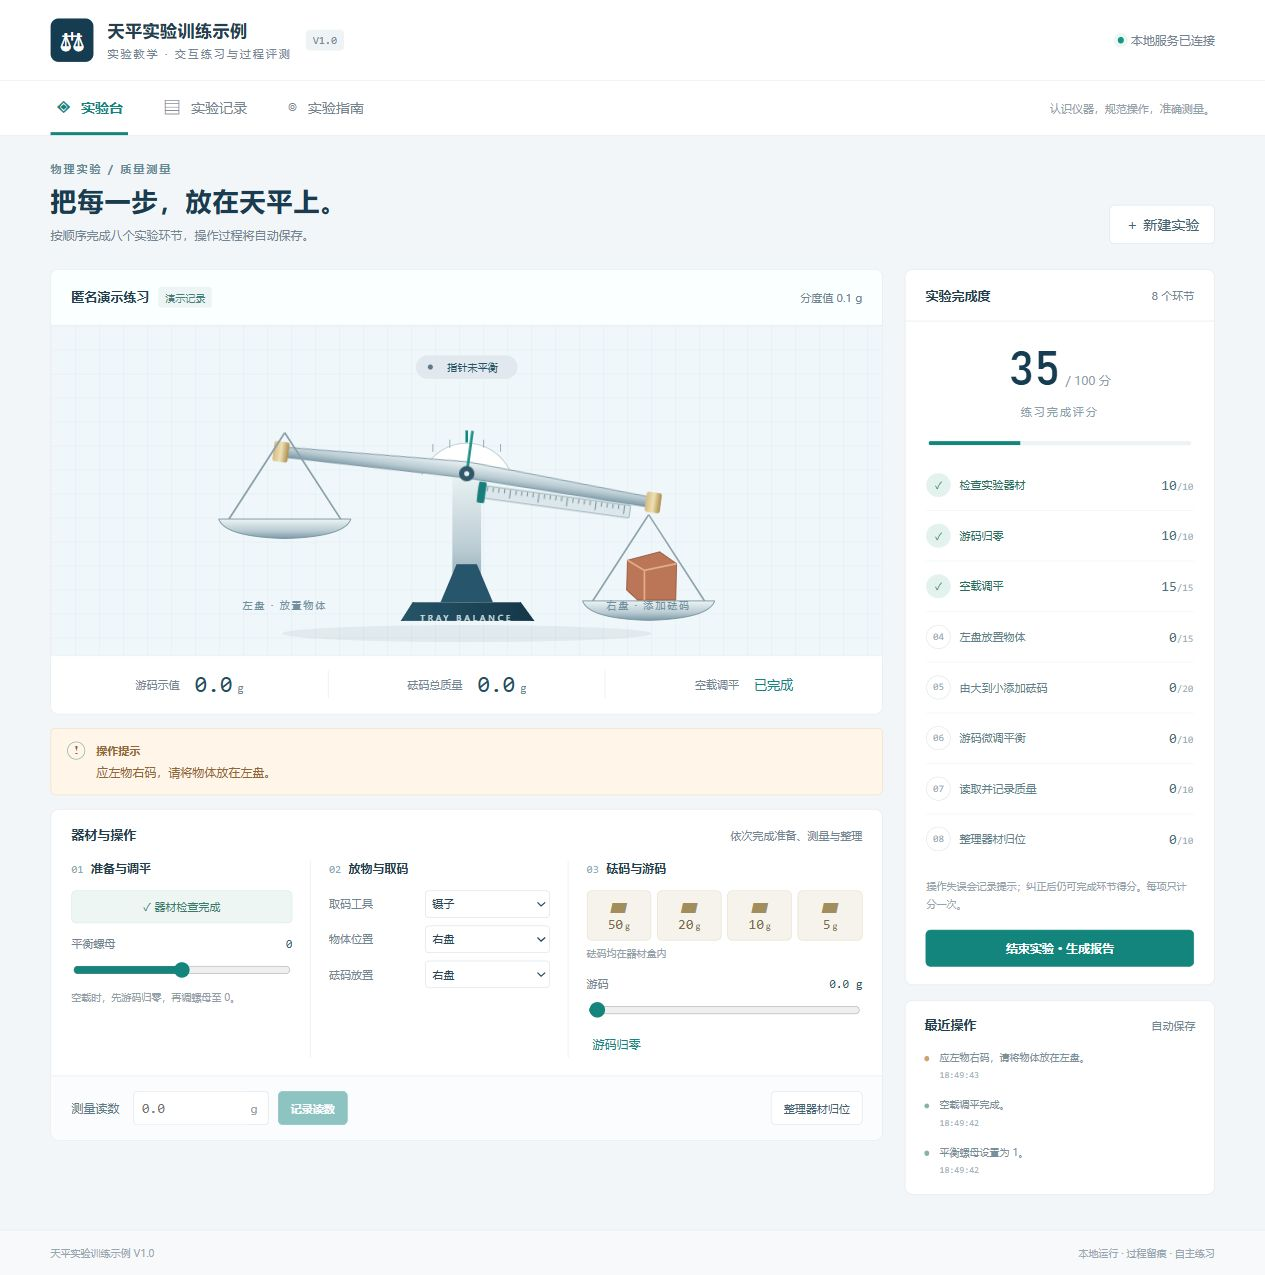
\includegraphics[width=0.95\linewidth,height=125mm,keepaspectratio]{03-error.png}
\caption{操作不规范时的反馈及过程记录}
\end{figure}

\begin{longtable}{@{}p{38mm}p{114mm}@{}}

\toprule

提示场景 & 修正方法 \\

\midrule

\endfirsthead

\toprule

提示场景 & 修正方法 \\

\midrule

\endhead

未归零或未空载调平 & 先取回器材，将游码归零，重新完成空载调平。 \\

物体或砝码位置不规范 & 将错误位置器材取回，再按左物右码放置。 \\

徒手取放砝码 & 切换为镊子后重新进行砝码操作。 \\

未平衡或读数错误 & 调整砝码及游码，平衡后计算并重新提交读数。 \\

\bottomrule

\end{longtable}

违规事件保留在过程记录中。纠正操作并取得相应分数后，历史事件仍保留，便于复查发生时间与提示内容。

\section{结束实验与查看报告}

\begin{figure}[!htbp]\centering
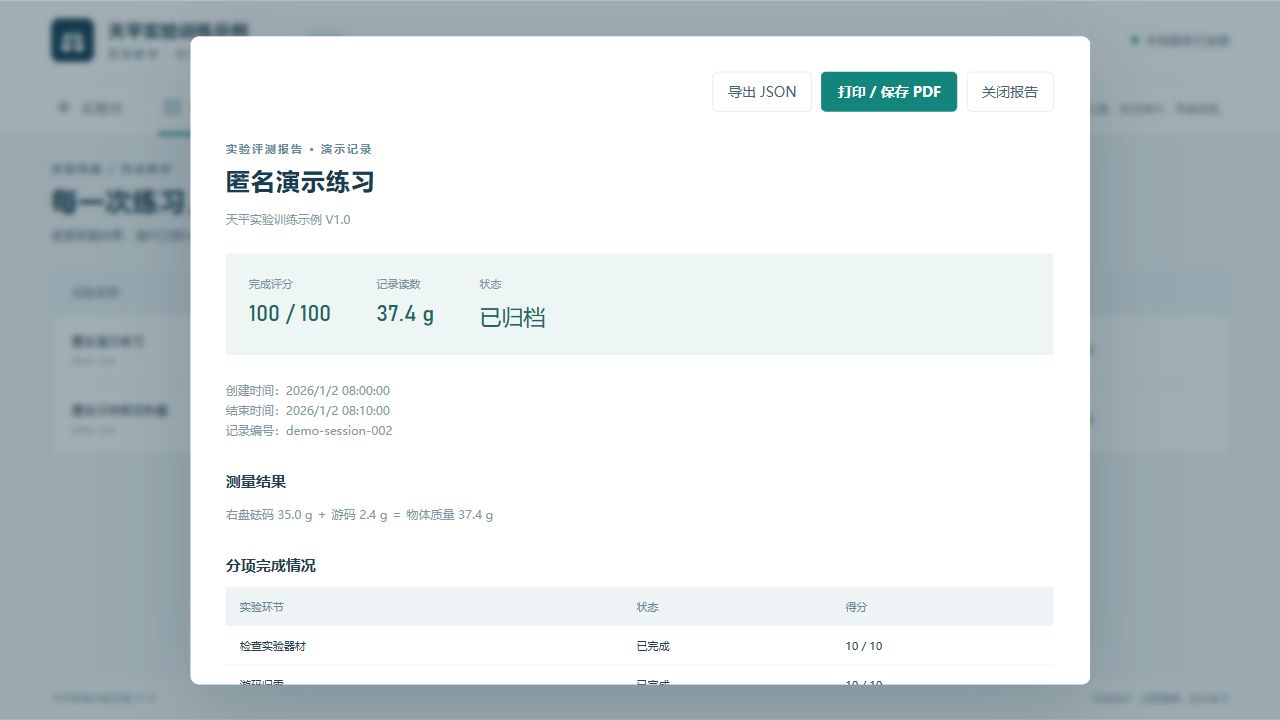
\includegraphics[width=0.95\linewidth,height=125mm,keepaspectratio]{05-report.png}
\caption{实验结果与练习报告}
\end{figure}

正确读数后执行器材整理，使物体与砝码回到收纳位置并将游码归零。完成收尾后结束本轮实验，查看累计得分、八环节结果、读数和过程记录。

\subsection{报告打印}

在报告界面调用打印功能，使用浏览器打印对话框选择“另存为 PDF”或本机 PDF 打印机，检查纸张和预览后保存。报告数据来自当前选中的实验轮次。

\subsection{重新练习}

重新开始时创建新的实验轮次，器材状态、得分和本轮事件恢复为初始状态。旧轮次保留在历史记录中，不会被新轮次的操作覆盖。已结束轮次用于查看，不继续接收操作。

\section{历史记录与数据导出}

\begin{figure}[!htbp]\centering
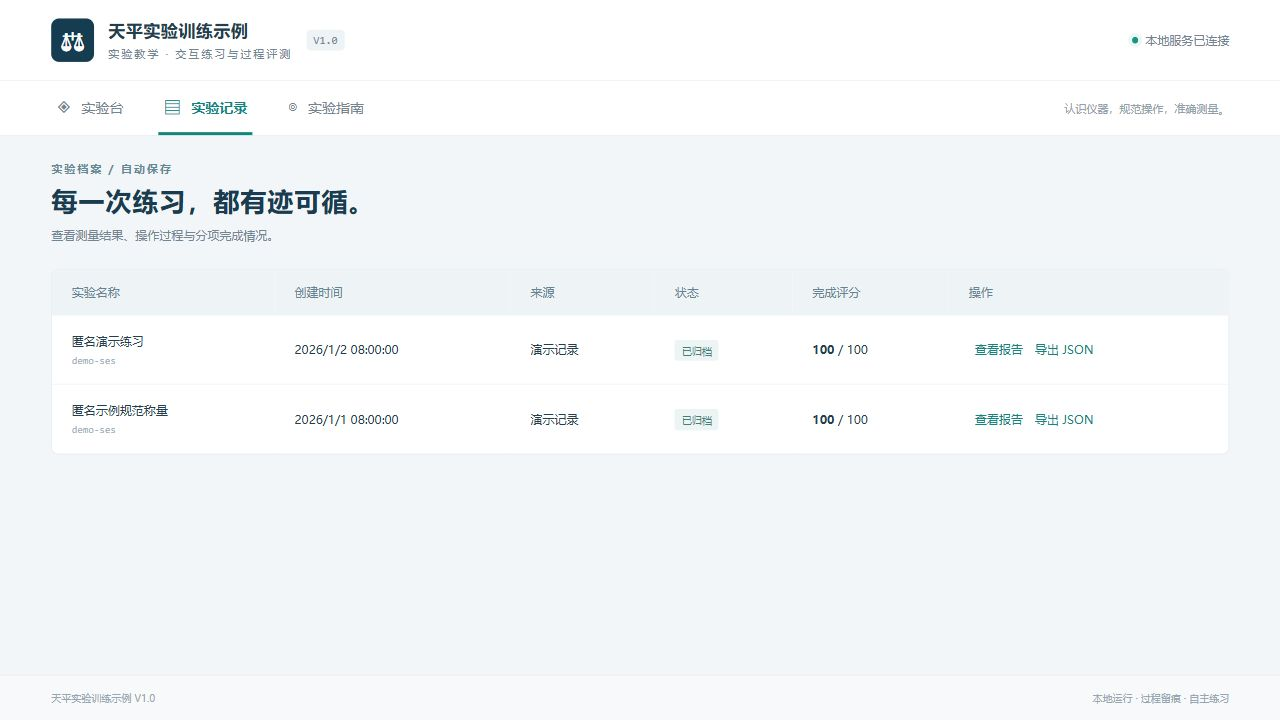
\includegraphics[width=0.95\linewidth,height=125mm,keepaspectratio]{06-history.png}
\caption{历史实验列表及记录查看入口}
\end{figure}

进入历史记录查看已保存轮次，依据名称、时间、来源和得分选择目标记录。打开详情后核对轮次标识，防止把不同练习的读数或报告混用。

\subsection{记录导出}

通过记录导出入口下载所选轮次的 JSON 文件。文件包含轮次信息、实验状态、分项结果及事件，可用于留档。JSON 为结构化数据文件，阅读时可以使用文本编辑器；当前版本不提供从该导出文件导入恢复的界面。

\subsection{演示数据}

带演示来源标记的轮次用于功能展示和证据留档，不代表真实学生的测试记录。用户自己的普通练习另建轮次，不沿用演示名称替代实际身份。

\section{操作指南与常见问题}

\begin{figure}[!htbp]\centering
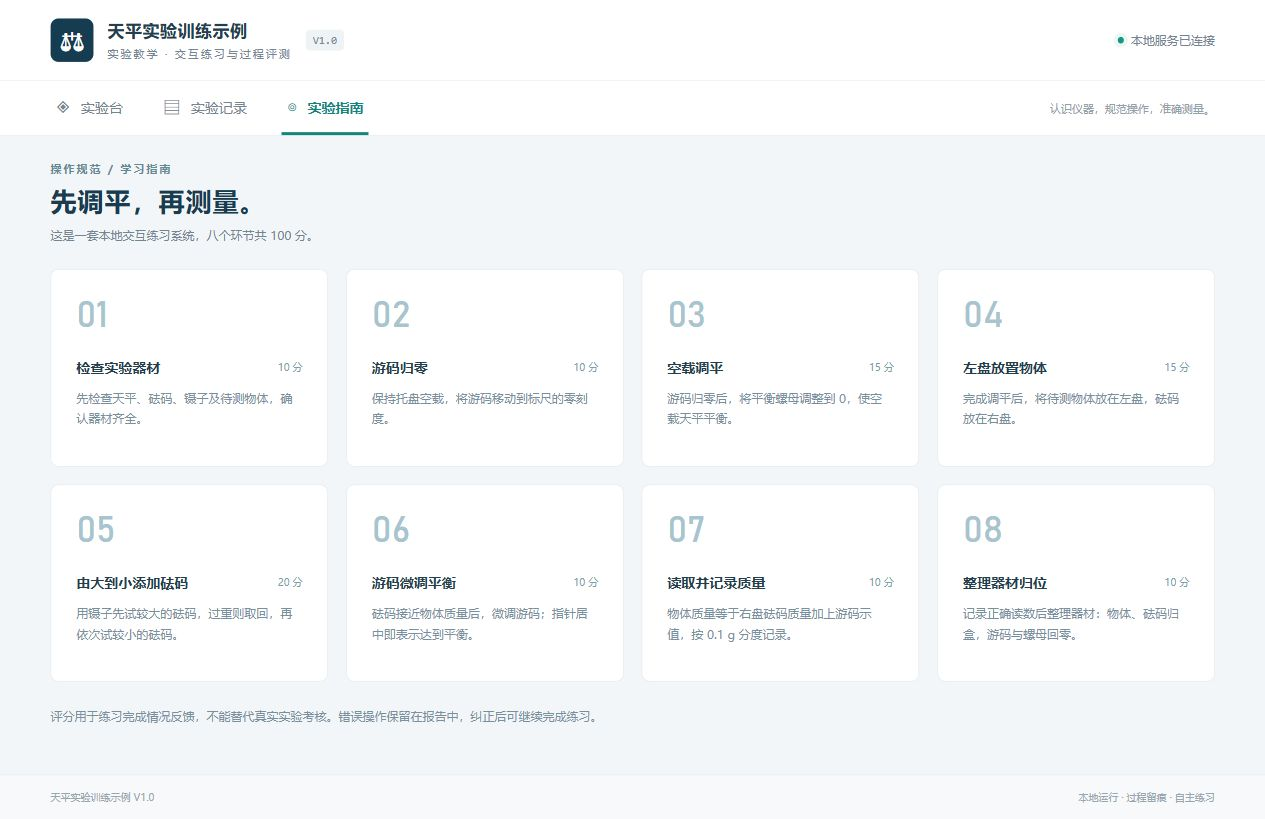
\includegraphics[width=0.95\linewidth,height=125mm,keepaspectratio]{07-guide.png}
\caption{系统内置操作指南}
\end{figure}

\begin{longtable}{@{}p{38mm}p{114mm}@{}}

\toprule

问题 & 处理 \\

\midrule

\endfirsthead

\toprule

问题 & 处理 \\

\midrule

\endhead

刷新页面后如何继续 & 先读取当前实验状态；以服务端保存结果为准，必要时从历史记录定位。 \\

页面无法连接服务 & 确认启动成功、访问地址正确，检查终端错误信息和端口占用。 \\

点击后没有得到预期分数 & 查看反馈，确认前置步骤、工具、托盘位置及平衡状态。 \\

需要迁移到另一电脑 & 停止服务后复制完整项目及数据目录，在目标电脑准备 Node.js 后启动。 \\

\bottomrule

\end{longtable}

\section{数据保存与软件结构}

系统由 React 与 TypeScript 前端、本机 Node.js HTTP 服务及 JSON 数据文件组成。前端负责呈现器材和接收输入；服务端验证请求、更新实验状态、计算得分并保存结果。前端不自行决定最终得分。

\begin{longtable}{@{}p{38mm}p{114mm}@{}}

\toprule

层次 & 职责 \\

\midrule

\endfirsthead

\toprule

层次 & 职责 \\

\midrule

\endhead

浏览器界面 & 呈现操作台、历史记录、指南及报告；提交动作并显示反馈。 \\

本机服务 & 处理健康检查、创建轮次、动作提交、状态查询、结束、历史及导出请求。 \\

本地存储 & 使用 JSON 保存轮次，通过串行写入与临时文件替换完成更新。 \\

\bottomrule

\end{longtable}

\subsection{保存与备份}

操作状态保存到项目本地数据目录。备份前先停止服务，再复制数据文件及必要程序文件。不要在服务运行时手工改写数据文件，也不要删除数据目录后期待历史记录仍能保留。

\subsection{隐私与访问}

服务仅绑定本机回环地址，不提供公网账号和跨设备协作。实验名称可使用课程或轮次描述，不必填写身份证号码、联系电话等个人信息。

本说明书适用于 V1.0。升级后应同步更新说明书和鉴别材料。
\end{document}
